% Please don't change anything in the documentclass below:
\documentclass[compsoc, conference, a4paper, 10pt, times]{IEEEtran}

% We recommend using these packages as below, but if you have a good reason and want to change these, you can.
\usepackage{cite}
\usepackage{amsmath,amssymb,amsfonts}
\usepackage{algorithmic}
\usepackage{graphicx}
\usepackage{textcomp}
\usepackage{xcolor}
\usepackage{booktabs}
\usepackage[hidelinks]{hyperref}

\usepackage[colorinlistoftodos, textsize=scriptsize]{todonotes}
\presetkeys{todonotes}{fancyline}{}
\newcommand{\jt}[1]{{\begin{textcolor}{red}{#1}\end{textcolor}}}

\usepackage{acronym}
\acrodef{BLXNS}{branch with link and exchange to non-secure state}
\acrodef{BUSted}{Microarchitectural Side-Channel Attacks on the MCU Bus Interconnect}
\acrodef{BXNS}{branch with exchange to non-secure state}
\acrodef{DCAP}{Data Center Attestation Primitives}
\acrodef{DHKE}{Diffie-Hellman Key Exchange}
\acrodef{DMA}{Direct Memory Access}
\acrodef{ECU}{Electronic Control Unit}
\acrodef{EDL}{Enclave Definition Language}
\acrodef{EDP}{Enclave Development Platform}
\acrodef{EPID}{Enhanced Privacy ID}
\acrodef{GCM}{Galois-Counter Mode}
\acrodef{HUK}{Hardware Unique Key}
\acrodef{IDAU}{Implementation Defined Attribution Unit}
\acrodef{IoT}{Internet of Things}
\acrodef{JWT}{JSON Web Token}
\acrodef{IAS}{Intel Attestation Server}
\acrodef{ISR}{Interrupt Service Routine}
\acrodef{KDF}{Key Derivation Function}
\acrodef{LOC}{line of code}
\acrodefplural{LOC}[LOCs]{lines of code}
\acrodef{MAC}{Message Authentication Code}
\acrodef{MMIO}{Memory-Mapped I/O}
\acrodef{NSC}{Non-Secure Callable}
\acrodef{OTP}{One-Time Password}
\acrodef{PCBAC}{Program Counter Based Access Control}
\acrodef{PCCS}{Provisioning Certificate Caching Service}
\acrodef{PCS}{Provisioning Certification Service}
\acrodef{PKI}{Public Key Infrastructure}
\acrodef{PSK}{Pre-Shared Key}
\acrodef{PTA}{Pseudo Trusted Application}
\acrodef{QE}{Quoting Enclave}
\acrodef{RTT}{round-trip time}
\acrodef{SAU}{Secure Attribution Unit}
\acrodef{SCF}{Side Channel Finder}
\acrodef{SDK}{Software Development Kit}
\acrodef{SEV}{Secure Encrypted Virtualization}
\acrodef{SG}{Secure Gateway}
\acrodef{SGX}{Software Guard Extensions}
\acrodef{SM}{Software Module}
\acrodef{TA}{Trusted Application}
\acrodef{TCB}{Trusted Computing Base}
\acrodef{TEE}{Trusted Execution Environment}
\acrodef{V2X}{Vehicle-to-Everything}
\acrodef{VSA}{Value Set Analysis}
\acrodef{WSN}{Wireless Sensor Network}






\begin{document}

\title{Securing TrustZone: Symbolic Execution for Side-Channel Analysis in
ARM-M Binaries}

% Submissions should be anonymized. See the CFP for details on how to anonymize your paper, including any references to your own work.
%\author{\em Anonymous Authors}

% The author information is skipped here, but can be used to include author information in the publication.
\iffalse
\author{\IEEEauthorblockN{1\textsuperscript{st} Given Names Surname}
\IEEEauthorblockA{\textit{Affiliation} \\
City, Country \\
email address or website URL}
\and
\IEEEauthorblockN{2\textsuperscript{nd} Given Names Surname}
\IEEEauthorblockA{\textit{Affiliation} \\
City, Country \\
email address or website URL}
\and
\IEEEauthorblockN{3\textsuperscript{rd} Given Names Surname}
\IEEEauthorblockA{\textit{Affiliation} \\
City, Country \\
email address or website URL}
%% IEEE format can accommodate up to six authors this way
}
\fi

\maketitle

\begin{abstract}
  \todo[inline]{todo}
\end{abstract}


%\begin{IEEEkeywords}
%component, formatting, style, styling, insert
%\end{IEEEkeywords}

%
% \section*{Preamble}
% 
% Confidential computing, with a focus on fortifying the integrity of code
% and data actively in use, has prominently embraced the deployment of
% \acp{TEE}, exemplified by technologies like ARM TrustZone. These
% \acp{TEE} leverage hardware capabilities to establish secure enclaves for
% applications, elevating the security posture. However, despite the robust
% security framework provided by \acp{TEE}, the persistent threat of
% side-channel attacks remains a formidable challenge, operating beyond
% conventional threat model boundaries. Successful exploitation of these
% attacks can compromise the default security assurances embedded in the
% underlying hardware.
% 
% In the realm of embedded systems, ARM microcontrollers have emerged as
% pivotal components. Their ubiquity in the embedded systems market can be
% attributed to their versatility, energy efficiency, scalability, industry
% support, and integration capabilities. These factors collectively make
% ARM-based solutions a preferred choice for a wide range of applications,
% contributing to their widespread adoption across various industries. Recent
% strides in enhancing the security of ARM microcontrollers have seen the
% integration of TrustZone, a technology designed to compartmentalize and
% secure sensitive computations. Nevertheless, ARM microcontrollers equipped
% with TrustZone have become enticing targets for side-channel attackers.
% This chapter explores this duality — the amalgamation of heightened
% security through TrustZone and the persistent vulnerability to side-channel
% attacks.
% 
% Building upon the side-channel detection tool~\cite{scfmsp}, this chapter takes a significant step forward to enhance
% the precision of our previous static analysis tool. It leverages a
% groundbreaking symbolic taint-tracking approach to conduct static analysis
% on ARMv8-M binaries, proactively identifying both timing and storage
% channels. We introduces \ac{SCF}\textsuperscript{ARM}, an advanced and
% precise side-channel analysis tool designed to identify information leakage
% stemming from timing side-channels, interrupt-latency attacks (commonly
% known as Nemesis), novel DMA-based attacks (referred to as BUSted), and
% unintended information flow within TrustZone applications tailored for ARM
% microcontrollers.  The evaluation results affirm the robustness and
% scalability of \ac{SCF}\textsuperscript{ARM} in detecting vulnerabilities
% within realistic applications, thereby establishing its effectiveness as a
% proactive measure for bolstering security in ARM-based confidential
% computing environments.

\section{Introduction} \label{sect:intro3}

With the rapid proliferation of \ac{IoT} devices across domains such as
smart homes, healthcare, transportation, and industrial systems, ensuring
the security of these interconnected devices has become an utmost concern.
\ac{IoT} systems, consisting of embedded devices and networked components,
handle an abundance of sensitive data, making them prime targets for
malicious actors who seek to exploit vulnerabilities to extract information
or gain control over installations~\cite{IOTSecurity1, IOTSecurity2}. Among
the multitude of security threats, timing side-channel attacks have emerged
as a significant and pervasive challenge. These side channels leverage
timing variations in program execution to compromise the confidentiality
and of sensitive data~\cite{timingattack, Nemesis, Cache1,
brumley2011remote, Travis, busted}.  

ARM-family processors have emerged as a dominant choice for embedded
devices, the \ac{IoT}, and mobile phones, capturing a substantial market
share of over 60\%\cite{arm_qualcomm}. To enhance security, ARM has
incorporated TrustZone~\cite{TZM, DemystifyingAT}, a hardware-based
\acp{TEE}, into their processors. TrustZone ensures the isolation of
security-critical software and data from the rest of the system, enabling
secure execution of critical tasks and protection of sensitive information.
It achieves this by dividing the processor into two separate and concurrent
security realms or worlds: the 'Normal World' and the 'Secure World.' These
worlds operate independently of each other, possessing distinct memory
spaces and execution environments. Thus, developers often rely on the
presumption that secrets are protected within the secure world due to the
processor's isolation guarantees.  However, research~\cite{surveyonTEE,
DemystifyingAT, loadstep, truspy, Bypassed, Qualcomm, busted} reveals the
potential vulnerability of the TrustZone secure world to side-channel
attacks that can lead to the unintended disclosure of secrets. 

%For instance, TruSpy \cite{truspy} exploits the cache contention between
%normal world and secure world to implement a timing-based cache
%side-channel attack and then extract a full 128-bit AES encryption key
%stored in the trusted environment. The research demonstrated that while
%the contents of the processor cache are safeguarded by the hardware
%isolation, the access pattern to these cache lines remains unprotected.
%Similarly, in \cite{Qualcomm}, researchers targeted Arm TrustZone in a
%malicious OS scenario. They leveraged the OS's capabilities to invoke
%interrupts and utilized the Prime+Probe \cite{primeandprobe} technique to
%recover a 256-bit private key from Qualcomm's ECDSA algorithm. %

The TrustZone technology employed in Armv8-M processors (such as
Cortex-M23/ M33/ M35P/ M55/ M85), do not claim to protect against
side-channel attacks~\cite{armdeveloper}. Primary attack vecturse here are
secret-dependent control flow with measurable timing differences or
secret-dependent memory access patterns.  Furthermore, TrustZone cannot not
effectively prevent secret leakage that stems from program implementation
flaws, which can arise from weaknesses in protocols or algorithms, as well
as mistakes made by developers.
%
\todo{add a few references here} 

%As an example, let's consider an One-Time Password \gls{OTP} system
%implemented within the TrustZone environment \cite{trustotp}. In a secure
%and well-implemented \gls{OTP} system, once an \gls{OTP} is utilized, it
%should immediately become invalid and should not be stored in any
%accessible location. However, if the \gls{OTP}s are stored in an insecure
%manner, such as being logged or stored in plaintext on unprotected memory
%or external I/O, an unauthorized attacker who gains access to the system
%or the logs could retrieve the previously used \gls{OTP}s. %

Early detection of side channel attacks enables proactive mitigation
measures to be implemented. Over the years, researchers and practitioners
have proposed various approaches to analyze binary code, or source code
employing techniques such as symbolic execution~\cite{binsec, pitchfork},
type systems~\cite{scfmsp, MantelAVR, Agat, barthe2014system}, and machine
learning~\cite{MLforSC}, among others~\cite{timingattack}. These approaches
aim to identify and mitigate timing side channel vulnerabilities targeting
different architectures. However, each approach carries its own limitations
and strengths, necessitating a thorough exploration of the existing body of
work in this field (refer to Section \ref{sec:related3}).

In this paper, we present a new and automated approach to detecting timing
side-channel leakage in ARM TrustZone-M programs, utilizing symbolic
execution-based analysis for the static verification. Our approach and tool
targets the ARM Cortex-M23 microcontroller, capitalizing on the
predictability of instruction execution times on hese microcontrollers.
Our objective is to ensure the absence of timing side-channel
vulnerabilities, interrupt-latency vulnerabilities (such as
Nemesis~\cite{Nemesis}), DMA-based attacks (referred to as
BUSted~\cite{busted}), and detect any undesired explicit and implicit
information flow, which is roughly equivalent to the concept of covert
storage channels in later literature~\cite{storagechannel}. This is
particularly relevant in the context of applications that are
compartmentalized into a security critical application part (such as
managing and using cryptographic credentials) and a less critical part
(such as sending and receiving network packets) to make use of the ARM
TrustZone. 

Our proposed approach is implemented in an automated tool, \tool{} to
statically detect the aforementioned vulnerabilities vulnerabilities in
ARMv8-M binaries. The primary objective of \tool{} is to track the flow of
secret information between the TrustZone's secure world and the non-secure
world, detecting and reporting any potential information leakages. \tool{}
stands for ``Side Channel Finder for ARM'' and is named after earlier tools
with similar abilities for the AVR and MSP430 platforms~\cite{scfmsp,
MantelAVR} but relies on different analysis techniques.  To the best of our
knowledge, \tool{} presents the first static analysis tool for side-channel
detection in ARMv8-M binaries, and addresses both timing and storage
channels. 

To establish the efficacy of our approach, we evaluate \tool{} on a set of
benchmarks that spanned a diverse range of synthetic benchmark programs
designed to unveil both typical and challenging structures of
secret-dependent control flow,
%
\todo{add ref to Hans' paper}
%
and by running \tool{} on code from the BUSted~\cite{busted} publication.
In summary, our contributions include:

\begin{itemize}
%
  \item{We present a novel approach that relies on symbolic execution and
static analysis to conduct sound information flow analysis in compiled
ARM-V8 programs. our approach is tailored to detect side-channel
vulnerabilities in applications compartmentalization with ARM TrustZone.}
%
  \item{We have implemented our approach in a tool \tool{}, which we
evaluae and show that our approach successfully detects  timing side
channel attacks, Nemesis attacks~\cite{Nemesis}, BUSted
attacks~\cite{busted}, and undesired direct and indirect information flow
to unprotected locations. Our results demonstrate a high precision and
scalability of \tool{}, making it useful for real-world security
assessments.}
%
  \item{We make \tool{} and our benchmark datasets publicly available under
an open-souce license at
\href{https://github.com/sepidehpouyan/ARM-SDFT}{https://github.com/sepidehpouyan/ARM-SDFT}
%
\todo{license? pipe this through \url{https://anonymous.4open.science/} for
the submission} }
%
\end{itemize}


%\section{Background and Problem Statement } \label{sect:problem}

\subsection{TrustZone on ARM Cortex-M}

ARM TrustZone is a hardware-based security technology developed by ARM Holdings \cite{DemystifyingAT, TZArchitecture}. TrustZone essentially divides the ARM processor into two distinct execution environments: the ``Normal World'' and the ``Secure World''. In fact, this system-wide approach assigns two virtual cores to each physical processor, together with the mechanism to securely switch between both realms. These environments are isolated from each other, and the Normal World is typically where the non-secure, general-purpose operating system and applications run. The Secure World, on the other hand, is a more trusted and isolated area where security-critical operations, cryptographic functions, and sensitive data can be processed and stored.

On ARM application processors (Cortex-A) \cite{TZA}, a separate processor mode known as the secure monitor handles secure context switching between worlds. However, on ARM microcontrollers (Cortex-M) \cite{TZM} lack a dedicated secure monitor software. Instead, essential mechanisms integrated into the core logic act as gatekeepers, facilitating the transition between secure and non-secure realms. These two worlds are rigidly separated at the hardware level and possess differing levels of privilege. Non-secure software is explicitly restricted from directly accessing resources in the secure world. This chapter focuses exclusively on TrustZone features for Cortex-M processors.

TrustZone technology for Armv8-M devices is tailored for ARM microcontrollers, specifically the Cortex-M series. It's been finely tuned for swift context switching and ultra-low power embedded applications. Leveraging specialized hardware integrated into Cortex-M cores along with a dedicated secure instruction set, TrustZone facilitates the establishment of multiple software security domains. These domains enforce strict access controls, allowing trusted software exclusive access to secure memory and I/O, all while maintaining optimal system performance.

\textbf{Armv8-M Architecture} typically features a set of 32-bit general-purpose registers (R0 to R12, Link Register (LR), Program Counter (PC)) and floating-point register (D0-D15) that are shared between secure and non-secure states. TrustZone-enabled Armv8-M microcontrollers have separate stacks for each security state, with the Stack Pointer (SP) being security-banked, meaning one instance exists in each state. The CONTROL register and some other special-purpose registers are also banked, and the core automatically switches between their instances during state transitions. ARMv8-M architecture introduces a new ISA with additional instructions and features, which enhances code density, reduces interrupt latency, and improves system performance. The architecture includes a two-stage pipeline for instruction execution, providing efficient handling of instructions.

\textbf{Memory space} in the Armv8-M architecture is also partitioned into secure and non-secure memory regions. The secure memory space is further divided into two types: secure and non-secure callable (\gls{NSC}). Secure addresses are exclusively allocated for memory and peripherals that can only be accessed when the core is executing in secure state. The program address, the address of the instruction currently executed, determines the security state of the processor. In contrast, non-secure addresses are designated for memory and peripherals accessible by all software running on the device, including both secure and non-secure components. \gls{NSC} represents a unique class of secure memory locations that facilitates the transition of software from a non-secure to a secure state, allowing for controlled and secure state changes. 

The security state assigned to each memory address are established through either the programmable Secure Attribution Unit (\gls{SAU}) or by an fixed Implementation Defined Attribution Unit (\gls{IDAU}). The \gls{SAU} is always available in Armv8-M cores, while the \gls{IDAU} is external to the core and the presence depends on the vendors implementation. In cases where both the \gls{IDAU} and \gls{SAU} are available within a system, the \gls{SAU}'s attributions take precedence, unless the \gls{IDAU} specifies a higher security attribute for a particular address.The \gls{SAU} can only be programmed in the secure state. 

In ARM TrustZone-M, the Nested Vectored Interrupt Controller (NVIC) has been enhanced to enable secure and non-secure configuration for each interrupt. The processor seamlessly handles interrupts based on its current security state. Notably, when a non-secure interrupt occurs during secure code execution, the processor securely manages the transition, preserving secure context data and preventing information leakage.

For \textbf{Transition} between two worlds, three new instructions have been introduced including secure gateway (\gls{SG}), branch with exchange to non-secure state (\gls{BXNS}), and branch with link and exchange to non-secure state (\gls{BLXNS}). The \gls{SG} instruction is employed for switching from the non-secure to the secure state. It is typically found at the start of a secure entry point's veneer, which consists of an \gls{SG} instruction followed by a branch to the secure world's function. The veneers are meant to reside in memory regions attributed to the \gls{NSC} by the linker. The \gls{SG} instruction serves several functions, such as setting the security level to secure, banking registers, and resetting bit[0] of the LR register to 0, indicating that the return will lead to a transition back from secure to non-secure. To return from the secure world to the non-secure world, as illustrated in Fig. \ref{fig:Ttansition}, the compiler employs the \gls{BXNS} instruction. This instruction initiates a branch or return to the non-secure program.

\begin{figure}
  \centering
  \medskip
  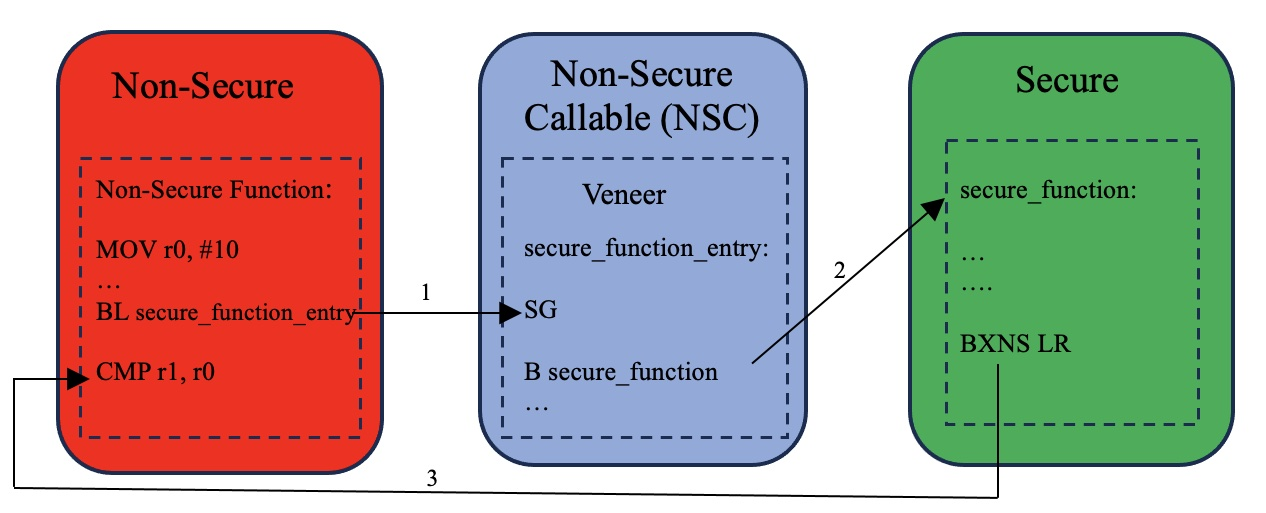
\includegraphics[width=.9\textwidth]{chapters/chapter3/image/SFC.jpg}
  \caption[Short caption for Table of Figures]{Secure Function Call in TrustZone-M}
  \label{fig:Ttansition}
\end{figure}

Conversely, secure software can invoke functions in the non-secure world. This action prompts the generation of compiler code that orchestrates the transition. It begins by preserving all registers, including the return address, within the secure stack. Subsequently, the registers are cleared. The \gls{BLXNS} instruction is used to execute the branch to the non-secure world, where it sets LR to a specific value, FNC\_RETURN (0xFEFFFFFF). Upon completion of the execution in the non-secure world, a return to the secure world is initiated using 'BX' instruction. When the BX instruction detects the FNC\_RETURN value in LR, it triggers a transition to the secure state. This shift is made possible by restoring all saved registers, including the return address, from the secure stack. It's also important to note that state transitions may also occur due to exceptions and interrupts.

TrustZone is not bullet-proof and has experienced successful attacks across various methods and contexts \cite{DemystifyingAT, surveyonTEE, returntononsecure}. The architecture, while designed to provide robust hardware-based security by isolating secure and non-secure worlds, is not immune to microarchitectural side-channel vulnerabilities \cite{DemystifyingAT, busted, surveyonTEE, truspy, Bypassed}. These vulnerabilities arise due to the shared resources and memory management between the secure and non-secure domains. Arm \cite{armdeveloper} has acknowledged that the security extensions for the Armv8-M architecture are not designed to protect against side-channel attacks resulting from control flow or memory access patterns. They argue that such attacks are not exclusive to the Armv8-M architecture and can apply to any code with secret-dependent control flow or memory access patterns. This type of attack can be mitigated by ensuring that the control flow and memory accesses patterns created by the program do not depend on secret state.

\subsection{Microarchitectural Side-Channel Attacks}

The security model proposed by \gls{TEE}s is not foolproof and must be approached with caution regarding side-channel attacks. These attacks aim to uncover confidential information hidden within the shared microarchitectural state during a victim's execution by exploiting observable side effects, notably timing variations. Typically, adversaries begin by initializing the shared microarchitectural elements in a predetermined state. They then proceed to measure state changes during or after the victim's execution, utilizing methods such as transactional memory aborts or performance monitoring counters. However, the most prevalent method for observing microarchitectural state changes is through timing analysis \cite{vanbulckphdthesis}. In cases where microarchitectural optimizations depend on global stateful elements like Translation Lookaside Buffers (TLB), caches, or branch predictors, any modifications to these elements during the victim's execution will result in measurable timing differences in the attacker domain. The analysis of microarchitectural state updates provides valuable insights into the victim's behavior, even in scenarios where attackers are architecturally isolated and have limited interaction with the victim, strictly through defined input and output channels.

Single-purpose embedded processors typically emphasize simplicity, power efficiency, and cost-effectiveness over advanced microarchitectural features like caches, pipelining, and speculative execution. This focus results in predictable instruction timings, reducing the risk of side-channel attacks. However, research \cite{Travis, brumley2005remote} has demonstrated that secrets can still be revealed through start-to-end timing side channels, by measuring the overall execution time of secret-dependent branches, even on processors with entirely deterministic instruction timing behavior. 

In addition, Nemesis-type interrupt timing attacks \cite{Nemesis} can exploit highly precise, instruction- granular timing measurements, which can even compromise secrets from branches with balanced start-to-end timings. These side-channel attacks abuse the CPU's interrupt mechanism to reveal microarchitectural instruction timings within \gls{TEE}s. The attack leverages the fact that hardware interrupts are only processed upon instruction retirement, after the currently executing instruction has completed, resulting in variable CPU cycles for different instruction types and processor states. Consequently, an untrusted operating system can precisely measure interrupt handling time, to retrieve the execution length of interrupted instruction and distinguish between secret-dependent program branches. In essence, for a successful Nemesis attack on processors with constant-time interrupt latency and multi-cycle instruction sets, where each instruction is uninterruptible, an attacker just requires a different execution time for at least one instruction in the if/else branch.

In recent findings, researchers have identified DMA-based side-channel attacks specifically aimed at embedded TEEs \cite{busted, marton}. These attacks exploit nuanced timing variations arising from contention between a DMA device and the CPU as they access the shared memory bus. This exploitation enables the attacker to construct a cycle-accurate memory access trace of a victim program. Notably, at the Black Hat Asia conference, Cristiano Rodrigues presented a side-channel attack that leverages DMA to target ARM TrustZone. This sophisticated attack effectively bypasses hardware-enforced isolation primitives, providing unauthorized access to Trusted Applications (\gls{TA}s) and resulting in the unauthorized leakage of sensitive information.

\subsection{BUSted: Microarchitectural Side-Channel Attacks on TrustZone-M MCUs}

BUSted \cite{busted} is a novel class of microarchitectural side-channel attacks that leverage the timing differences exposed in the arbitration logic of the MCUs bus intecconnect. It's evident that concurrent access by multiple bus master (e.g., CPU, DMA) to a shared bus slave (e.g., memory controller) leads to time delays for at least one, causing subtle timing variations. By observing the timing drifts on memory transactions, an attacker can extract information regarding the victim’s memory access pattern. Consequently, without breaking security isolation boundaries, a malicious bus master can spy on bus activity and determine when another bus master accessed a specific slave.

ARM adopts a load-store memory access model, restricting memory interaction solely to load/store (LDR and STR) instructions. Thus, an attacker can exploit the MCU's load-store architecture to observe timing variations. Specifically, in cases where the victim code incorporates secret-dependent control flow and loads/stores execute at different clock offsets on conditional paths, this discrepancy leads to distinct memory access patterns. An attacker could exploit this to deduce and illicitly obtain a particular secret.

To elaborate further, let's examine a code snippet (compiled for the Arm Cortex-M23) that includes a balanced conditional statement dependent on a secret variable, as visualized in Fig. \ref{fig:busted}. Since both execution paths have an identical execution time of 5 clock cycles, starting from t + 1 after the \textit{cmp} instruction, an attacker wouldn't observe any difference in execution time. Consequently, distinguishing between these execution paths and subsequently extracting the secret becomes unfeasible. Yet, an observer could still detect divergent memory access patterns between these two execution paths. When the branch (\textit{bne}) isn't taken, it completes within a single clock cycle, causing the \textit{str} instruction to occur at clock cycle t + 3. Conversely, if taken, the branch incurs a two-clock-cycle process, resulting in the \textit{str} instruction taking place at clock cycle t + 4. Overall, this changes the relative position of the \textit{str} instruction to the \textit{bne} instruction and unveils the secret. By monitoring either 't + 3' or 't + 5' clock cycles, an attacker can potentially deduce the secret by observing the presence or absence of contention on the data memory bus.

\begin{figure}
  \centering
  \medskip
  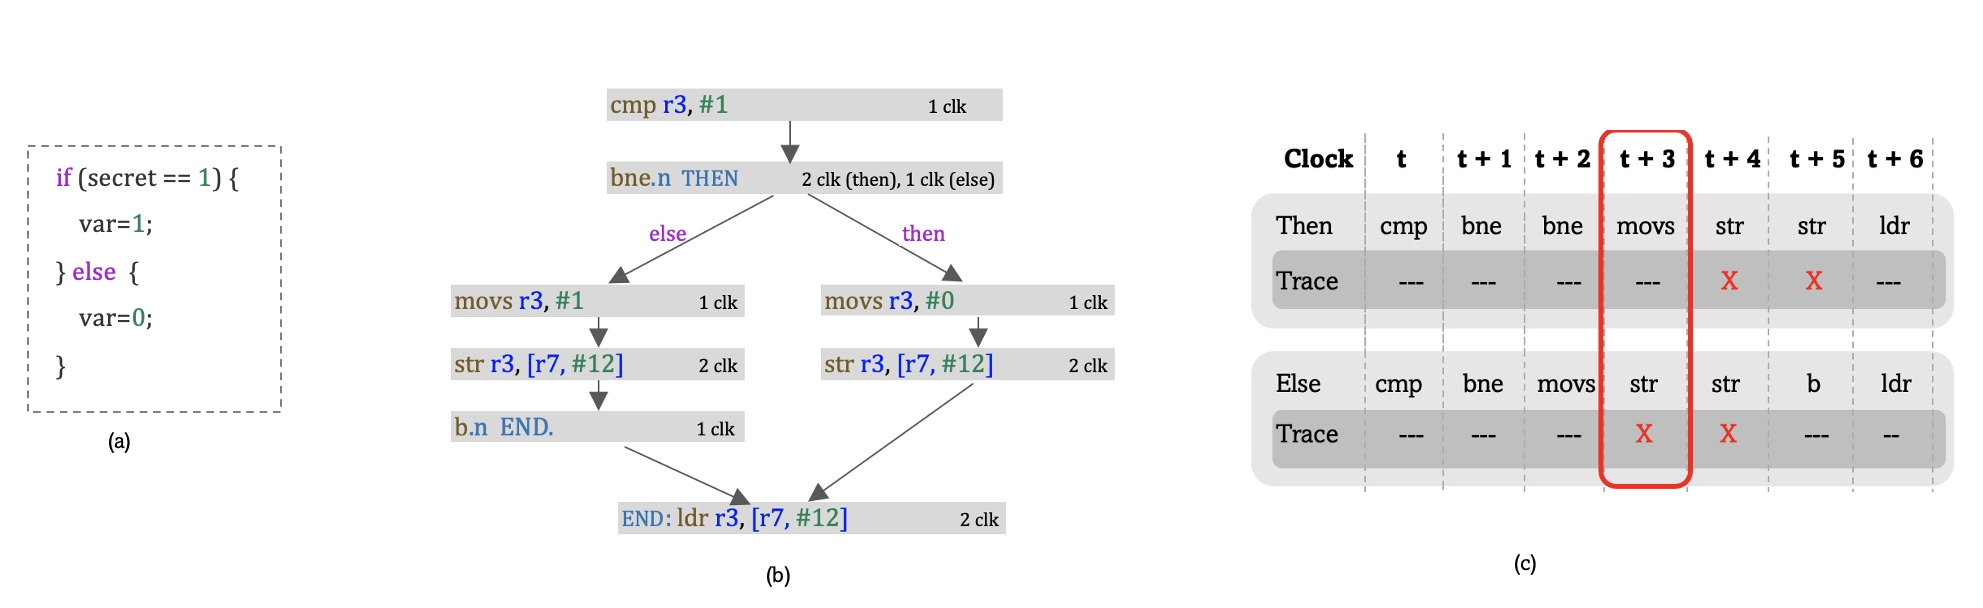
\includegraphics[width=.9\textwidth]{chapters/chapter3/image/busted.jpg}
  \caption[Short caption for Table of Figures]{(a) secret-dependent branch, (b) compiled code CFG for Arm Cortex-M23, (c) memory access pattern and monitoring of clock t+3 and t+5.}
  \label{fig:busted}
\end{figure}

Given the nature of this attack, targeting on microarchitectural design issues, comparisons have arisen likening its impact to that of renowned exploits like 'Spectre' and 'Meltdown' which affected more complex architectures in recent history. Embedded projects relying on hardware-assisted privilege separation via TrustZone-M must now factor in the potential for information leakage from secure components operating within the secure world. According to the researchers, there are software-based countermeasures available to mitigate the impact of this microarchitectural design flaw. The crucial consideration in addressing time-based attacks involves minimizing the presence of secret-dependent code in security operation implementations. Essentially, the time required for a security procedure should remain independent of the success or any secret of the operation.

\subsection{Covert Storage Channels}

Sensitive information can be unintentionally leaked through covert storage channels \cite{storagechannel, sabelfeld}. These channels, whether explicit or implicit, provide pathways for the unauthorized transfer of sensitive data, which can compromise system security. Implicit covert storage channels, in particular, introduce challenges, as data can inadvertently traverse indirect or unintended pathways resulting from the program's control structure. This contrasts with explicit information flows, which occur when confidential data is directly assigned to public variables. To illustrate, let us consider a scenario with two security levels: ``high'' and ``low,'' denoting varying degrees of confidentiality. We can examine the code presented in Fig. \ref{fig:implicit}, which exhibits a data flow from the high variable \textit{h} to the low variable \textit{l}. The insecurity within this code stems from the \textit{l = 1} assignment in a control context conditioned upon the confidential variable \textit{h}.

 \begin{figure}
  \centering
  \medskip
  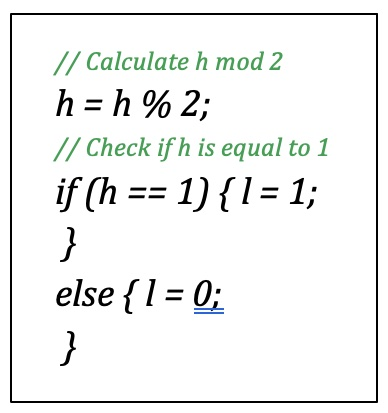
\includegraphics[width=.3\textwidth]{chapters/chapter3/image/implicit.jpg}
  \caption[Short caption for Table of Figures]{An implicit information flow}
  \label{fig:implicit}
\end{figure}

\subsection{Static Code Analysis}

\textbf{Taint Analysis} stands as a crucial program analysis method, meticulously tracing the flow of data of interest throughout program execution. Taint analysis utilizes 'taint tags' as markers attached to registers and memory, serving to indicate their taint status. It operates via three integral components:

\begin{enumerate}
  \item[1.] Taint Sources: These denote points within the program or memory locations where relevant data is introduced, often focusing on user inputs from local or remote sources.
  
  \item[2.] Taint Propagation: This involves the transfer of taint tags during program execution, governed by predefined rules aligned with instruction semantics. Consider the instruction ADD src, dst; in this scenario, a taint propagation rule might dictate that the resulting tag of destination (dst) comprises a bitwise OR operation between the tags associated with src and dst.
  
  \item[3.] Taint Sinks: These specific program instructions serve as checkpoints for taint analysis, assessing the presence of targeted taint tags. They play a critical role in security applications, detecting potential threats like control flow hijacks or information leaks, often associated with control flow transfers or output system calls.
  
\end{enumerate}

\textbf{Value Set Analysis} operates as a static program analysis technique, approximating the potential values that each program data object might hold at any given program point. By analyzing individual instructions within a control-flow graph (CFG), value set analysis effectively tracks and estimates the diverse range of values that each data object could hold. 

\textbf{Symbolic Execution} stands as a method to explore the potential paths of program execution by substituting variables with symbolic representations. It systematically traverses the program, executing with symbolic inputs to understand the possible behaviors and identify vulnerabilities or paths that might lead to critical issues.

%\section{Static Information Flow Analysis} \label{sect:design}
%
\subsection{A Simple Example}

While TrustZone technology in Armv8-M processors offers robust security measures, it remains susceptible to side channel attacks due to secret-dependent control flow, resulting in observable timing variations or secret-dependent memory access patterns \cite{armdeveloper}. Furthermore, it's worth noting that TrustZone might not entirely mitigate implicit and explicit information leaks resulting from unintentional developer errors in secure coding practices, system architecture flaws, and non-compliance with stringent security standards and protocols.

To elaborate, consider a secure One-Time Password (\gls{OTP}) system illustrated in Fig. \ref{fig:OTP}. \gls{OTP} system is integral in verifying mobile users accessing critical web services that require a heightened level of security. An \gls{OTP} is a dynamically generated numeric or alphanumeric string of characters used to authenticate a user for a single transaction or session with an authentication server. This approach augments the traditional user ID and password authentication by introducing a dynamic password that changes with each authentication attempt. The \gls{OTP} mechanism operates by generating a code using an internal clock (or counter) and a factory-encoded secret key known as the 'seed.' 

To maintain the confidentiality of both the generated \gls{OTP}s and the associated seeds, the code and data involved in \gls{OTP} operations inhabit a secure enclave within TrustZone \cite{trustotp}. This enclave establishes a isolated space, distinct from the regular operating system running in the normal world. TrustZone technology guarantees the integrity and confidentiality of \gls{OTP}s and seeds by restricting access exclusively to the secure domain.

However, any inadvertent mishandling of the seeds or \gls{OTP}s—such as storing them in plaintext on unprotected memory, logging them, or exposed via non-secure I/O —or if an implicit flow is triggered by updating a publicly observable variable within the program control flow—an attacker could potentially access the generated \gls{OTP}s. Furthermore, the attacker might deduce secrets by analyzing time variations within a secret-dependent branch.

\begin{figure}
  \centering
  \medskip
  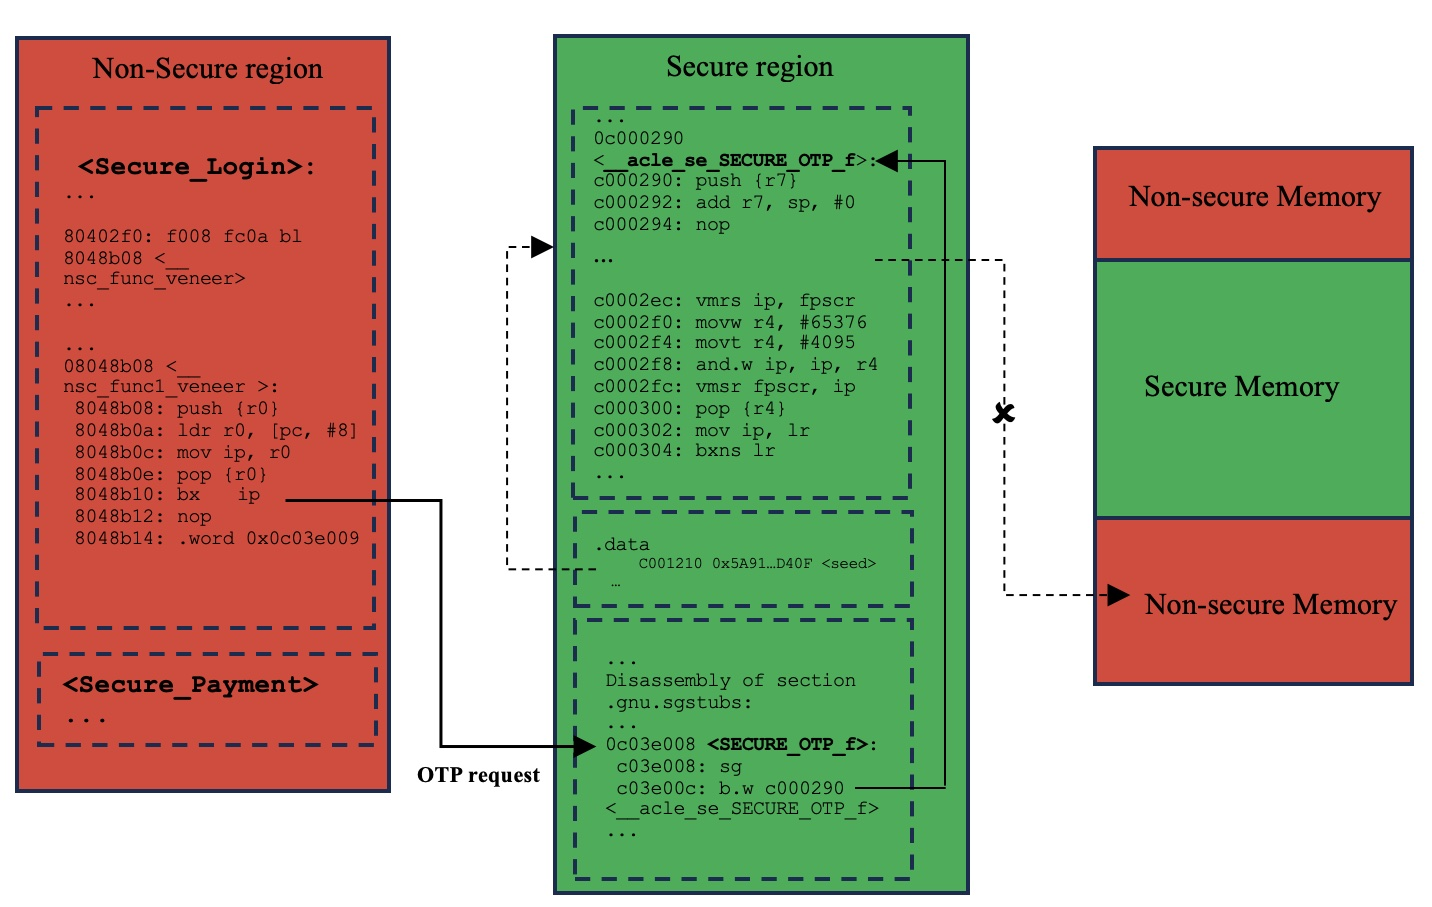
\includegraphics[width=.9\textwidth]{chapters/chapter3/image/OTP.jpg}
  \caption[Short caption for Table of Figures]{TrustZone-based Implementation of Secure OTP Generation}
  \label{fig:OTP}
\end{figure}

We present an approach that merges taint tracking techniques with symbolic execution of trusted application (\gls{TA}) binaries to systematically identify the undesired information leakage. Subsequently, we notify developers and designers of these identified leakage points for further action and resolution. 

\subsection{Scope and Threat Model}

\textit{Scope.} Our focus revolves around small-scale embedded systems and IoT devices that operate using MCUs, such as the Arm Cortex-M family. These MCUs operate within strict constraints, characterized by limited computing power and memory. They feature simplified microarchitectures, lacking components like caches and typically operating with 2-3 pipeline stages. Additionally, they do not support virtual memory. Generally, MCUs consist of a single CPU while offering a diverse array of peripherals, including UART, SPI, timers, DMAs, and I2C, among others. Some devices may incorporate MPUs, and the latest iterations of Armv8-M MCUs introduce support for dual security states, namely secure and non-secure worlds (known as TrustZone-M). These MCUs are engineered to ensure highly predictable outcomes, consistently delivering identical outputs for specific inputs within defined timing constraints.

\textit{Threat model.} The adversary’s goal is to extract sensitive information from an isolated environment by bypassing the memory isolation security mechanisms in TrustZone. We assume the attacker has access to either the source code or compiled binary code of the victim's program. Additionally, they can monitor the program's execution time and outputs. Furthermore, we consider a more capable attacker who has complete control over the unprotected normal world and its resources. This includes the ability to manage bus masters (e.g., DMA), configure peripherals like timers, and control scheduling decisions. We are not considering side channels arising from cache contention or branch prediction feature, as they fall beyond the scope of this work due to their absence in the targeted MCU architecture.

\subsection{Taint Tracking of Function Inputs}

Our method involves an information flow analysis that links each value with a security tag indicating its sensitivity level. We primarily categorize these levels into two labels: '\textit{H}' for high sensitivity and '\textit{L}' for low sensitivity, where '\textit{H}' signifies higher sensitivity than '\textit{L}'. Each input (initial state of registers, etc.) and output (final state of registers, etc.) of a program is assigned one of these labels. To effectively track and identify both explicit and implicit data flows of high sensitivity during program execution, our approach incorporates an effective symbolic taint-tracking mechanism.

Specifically, initial register contents and associated memory are transparently substituted with unconstrained symbolic values. We, furthermore, utilize Angr\footnote{https://angr.io/}’s annotation system to flag highly sensitive symbolic values as tainted. This taint, conservatively propagated throughout symbolic execution, allows for convenient querying during subsequent analysis to identify potential information leakage. 

\subsection{Timing-Sensitive Information Flow Policy}

An information-flow analysis verifies the absence of undesired information leakage within a program. A timing-sensitive variant of this analysis considers the impact of confidential data on the program's execution time. The intended security assurance is typically defined through information flow policies that prevent secret data from affecting an attacker's observations. This study utilizes a symbolic taint-tracking strategy to monitor potential policy violations during execution.

To this end, taint tags follow Angr's propagation rules during symbolic program execution, aligning with ARMv8-M instruction semantics. For example, in the case of an instruction like ‘ADD dst, src1, src2’, a taint propagation rule might dictate that the resulting tag of 'dst' is determined by performing a bit-wise OR operation on the tags of ‘src1’ and ‘src2’. Specifically, these rules imposes constraints on the sensitivity of data stored in registers and memory cells throughout program execution, affecting their state upon program termination. 

\subsection{Detection of timing side channels}

To ensure the absence of timing side channels within a program, our approach involves the initial computation of control-dependence regions for each branch instruction dependent on secret data. This computation employs the Safe Over-Approximation Properties (SOAPs) as defined in \cite{MantelAVR}. In particular, our focus lies in comparing the execution times between the 'then' and 'else' branches, distinguishing two distinct control-dependence regions for jumps influenced by confidential information.

Afterward, we sums up the execution time of all instructions within each region following the \textit{Definition} \ref{def:timing}. In scenarios where a nested branch \textit{br1} exists within the region of another branch \textit{br0}, a recursive procedure becomes necessary due to only one path of \textit{br1} being executed, whereas the positive part of \textit{Definition} \ref{def:timing} accounts for both paths' cumulative execution time. We address this by subtracting the execution time of the 'then' branch of \textit{br1}.

\newtheorem{definition}{Definition}[section]
\begin{definition}\label{def:timing}
    The function \textbf{branchPathTime\textsuperscript{r}} is defined recursively as: \\
    
   \centerline{$branchPathTime^r(br) := \Sigma (execution\_time(ins) - branchPathTime^{then}(ins))$}

   Where:
\begin{align*}
& \bullet \quad r \in \{ \text{then}, \text{else} \} \\
& \bullet \quad br \in \{ \text{beq}, \text{bne}, \text{bgt}, \text{blt}, \text{bge}, \text{ble} \} \\
& \bullet \quad \forall \text{ins} \in \text{region}^r(br)
\end{align*}

\end{definition}

Within ARMv8-M architecture, conditional branch instructions require an extra clock cycle when they are taken. With this fact, if the total time required for executing the 'then' region plus one equals the time taken for jumping and executing the 'else' region in a secret-dependent branch, it becomes impossible to discern the value of secret data by observing the program's overall execution time.

Furthermore, identifying the Nemesis vulnerability in an ARMv8-M binary involves pinpointing a jump instruction depending on secret data. Due to the variable execution times of branch instructions in ARMv8-M architecture when taken or not, an attacker can interrupt a branch instruction to capture the secret information. Consequently, the attacker can even execute a Nemesis attack on balanced paths.

To detect the BUSted vulnerability in a binary, we meticulously traverse every path within a branch dependent on secret information, scrutinizing the execution points of 'str' or 'ldr' instructions. If these instructions execute at different clock offsets on conditional paths, it exposes a potential vulnerability for attackers to exploit distinct memory access patterns and gain access to sensitive information.

\subsection{Augmented Taint Flow Directives}

Secret-dependent branches introduce variations in the program flow based on confidential information. By observing changes in execution time, logical operations, or other side channel information arising from these branches, attackers can deduce details about the secret data, such as its value or structure. Consequently, when a secret-dependent branch involves an operation where a memory cell or register is written within a particular path, it's crucial to mark that register or memory as tainted. These elements carry highly sensitive information during program execution, causing variations that attackers can exploit to infer the secret.

We employ Angr’s MemoryMixin extension, which conducts exhaustive validations on every memory access. Specifically, when these accesses occur within secret-dependent branches, we annotate the potentially symbolic values as tainted to reflect their elevated sensitivity within that particular context. This approach guarantees the absence of flows from secret information to attacker-observable outputs.

%\section{\ac{SCF}\textsuperscript{ARM}: DESIGN AND IMPLEMENTATION}

We have developed the \ac{SCF}\textsuperscript{ARM} specifically for the static analysis of ARMv8-M binaries targeting Cortex-M23, focusing on identifying timing side-channel vulnerabilities. Our approach, centered around symbolic taint-tracking, enables a rapid, cost-effective, and automated assessment of these vulnerabilities. We have implemented an open source  version of \ac{SCF}\textsuperscript{ARM} built upon Angr\footnote{https://angr.io/} and \ac{SCF}\textsuperscript{MSP} \cite{scfmsp}. Specifically, (1) we use Angr for symbolic execution of binaries and conducting Value Set Analysis (\ac{VSA}) to determine potential register values or symbolic memory addresses; (2) we expand the functionality of the \ac{SCF}\textsuperscript{MSP} tool to analyze TrustZone-M targeted binaries and ensure program integrity against a novel DMA-based side-channel attack termed BUSted \cite{busted}. 

Fig. \ref{fig:SCFARM} showcases a high-level workflow diagram detailing the components of the \ac{SCF}\textsuperscript{ARM} tool. The dashed box denotes the core elements implementing our proposed side channel evaluation technique. \ac{SCF}\textsuperscript{ARM} is built on approximately 1110 lines of Python code and integrates various established Python libraries, as detailed in the following.

\begin{figure*}
  \centering
  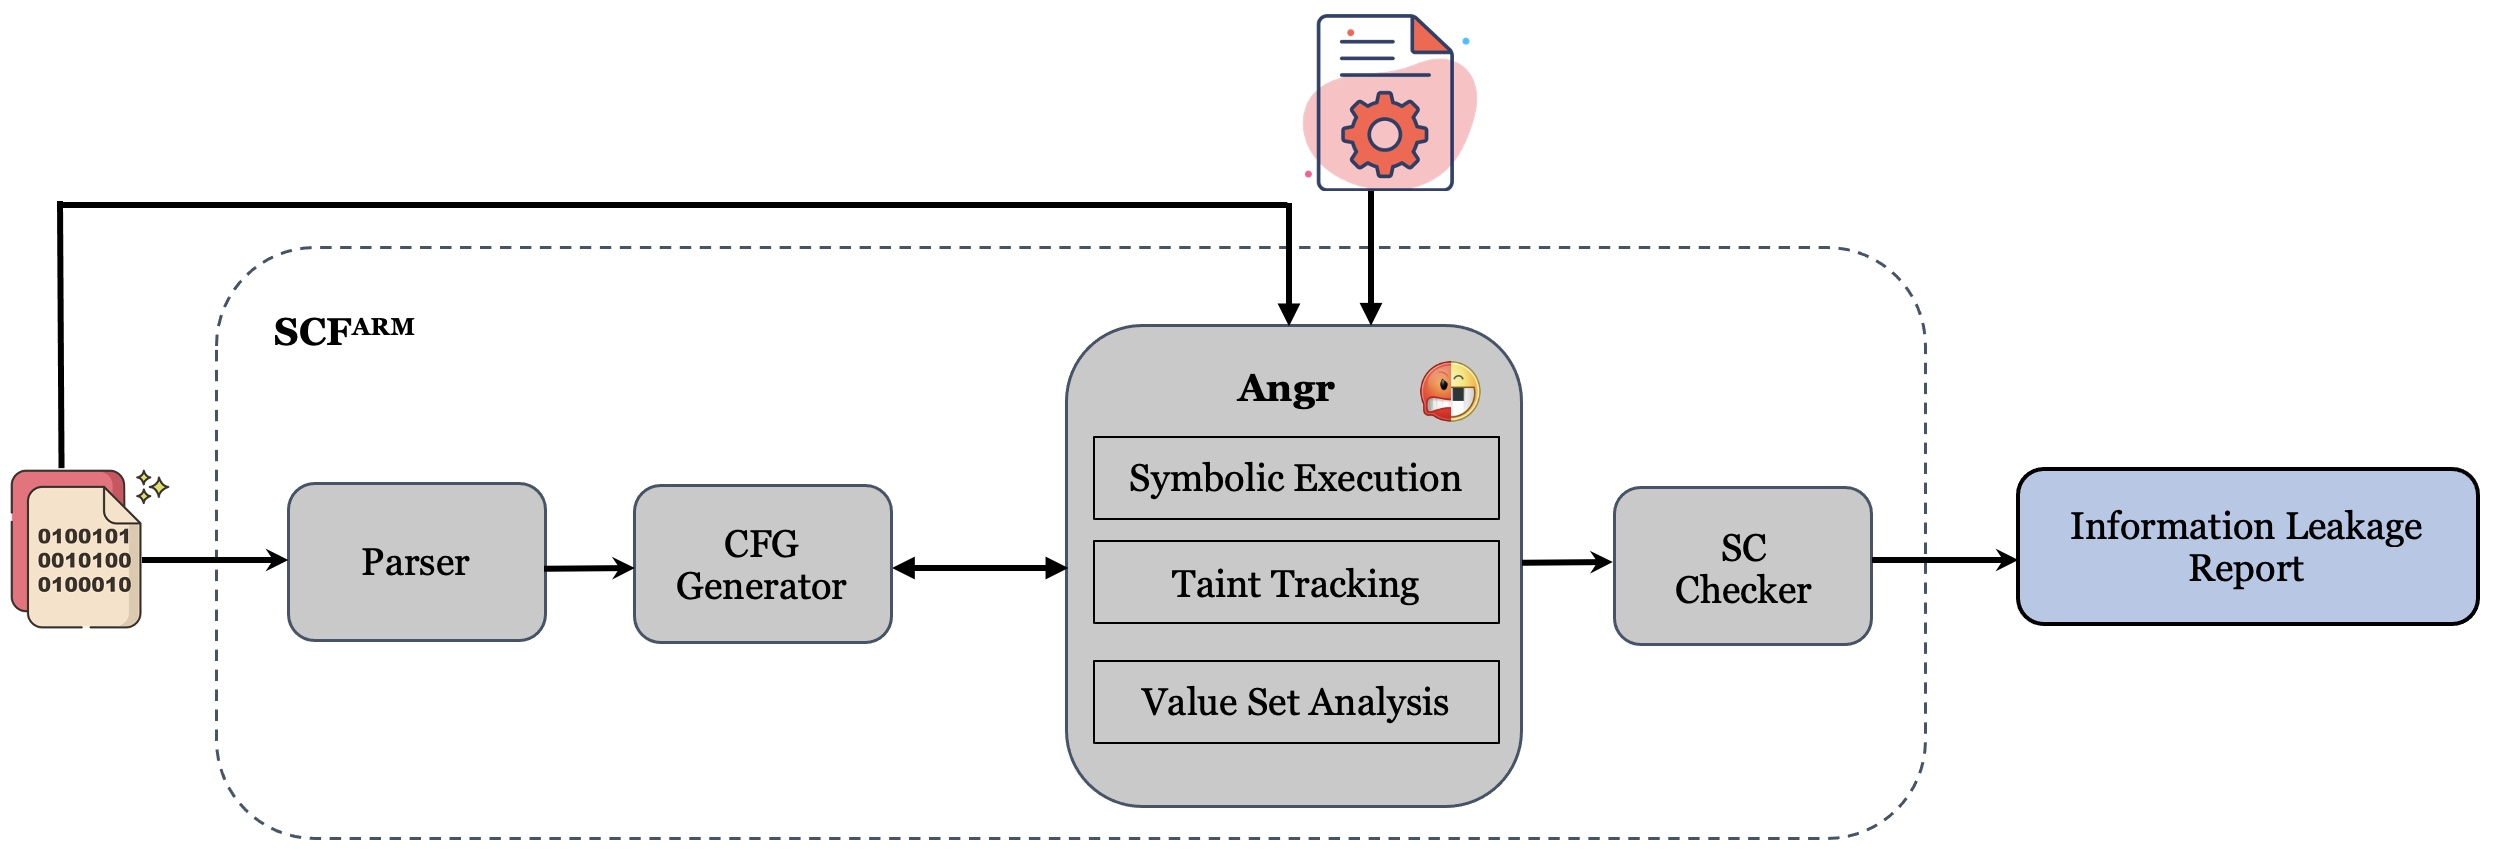
\includegraphics[width=.9\textwidth]{figures/SCFARM.jpg}
  \caption{Overview of \ac{SCF}\textsuperscript{ARM}}
  \label{fig:SCFARM}
\end{figure*}

We'll now provide a concise summary of each element and their practical implementations:

\textbf{Parser.} We employ this component to convert the input binary into assembly language. Initially, we utilize the pyelftools\footnote{https://github.com/eliben/pyelftools} Python library to locate the starting point of instructions within the binary. Subsequently, we leverage the Capstone\footnote{http://www.capstone-engine.org/} disassembler to translate the binary into ARMv8-M instructions, generating mnemonic codes and symbolic representations of processor instructions. This disassembly process allows us to extract essential details such as opcodes, addresses, and instruction lengths. Finally, we determine the required clock cycles for executing each instruction based on the specifications outlined in the ARMv8-M Architecture Reference Manual \cite{armv8m_ref_manual}.

\textbf{CFG Generator.} This component is responsible to construct an accurate program Control Flow Graph (CFG) using the NetworkX \cite{networkX} Python library. This component establishes a mutual connection with the subsequent component, enabling the retrieval of the target address for ‘branch and exchange’ instruction \textit{BX <Rm>} through \ac{VSA} in Angr. The resulting graph facilitates the identification of execution point predecessors and successors, aiding in computing control dependence regions for branches and inferring loops within assembly programs.

\textbf{Angr.} Utilizing a JSON-formatted configuration file that lists the starting function's arguments derived from high-level code to determine taint sources (i.e., highly sensitive inputs). This component employs Angr's annotation system to mark registers and memory cells containing confidential data with a taint label. It associates arguments with their corresponding registers following the ARMv8-M calling conventions \cite{armv8m_ref_manual}. These taint tags propagate during the symbolic execution of the input binary. Our taint analyzer tracks both explicit and implicit flows. Upon completion of symbolic execution, the component presents a list of tainted registers and memory cells for subsequent analysis. 

\textbf{SC Checker.} This module performs static analysis to identify potential side channel leaks within ARMv8-M assembly programs. Our \ac{SCF}\textsuperscript{ARM} tool currently detects vulnerabilities falling into four distinct classes:

\begin{itemize}

\item Timing Channel: Detected when a program exhibits different execution times depending on the secret input. \ac{SCF}\textsuperscript{ARM} detects these leaks by measuring the overall running times of if/else regions within the secret-dependent branches.

\item BUSted Vulnerability: Recognized when a program includes store/load instructions with different time offsets inside the if/else regions of a secret-dependent branch.

\item Nemesis Vulnerability: Identified when a program displays varying execution times for at least one instruction within the if/else regions of a secret-dependent branch.

\item Storage Channel: Flagged if there is an undesired information flow from secret inputs to observable output, such as return registers or non-secure memory.

\end{itemize}

%\section{EVALUATION AND DISCUSSION}

In this section, we present our assessment of \gls{SCF}\textsuperscript{ARM}, emphasizing the accuracy of our static analysis in detecting side channels. Our evaluation of \gls{SCF}\textsuperscript{ARM} included a thorough examination of a carefully selected set of benchmarks, influenced by \cite{hans}, featuring a diverse range of programs, from those with vulnerabilities to benign ones. These benchmarks were specifically designed to reveal typical and intricate patterns in secret-dependent control flow, providing a comprehensive examination of \gls{SCF}\textsuperscript{ARM}'s effectiveness. 

The benchmarks consist of C programs compiled using 'arm-none-eabi-gcc,' a cross-compiler toolchain tailored for generating code targeting ARM Cortex-M and Cortex-R processors without an operating system (bare-metal). The compiler is configured with the '-mcpu=cortex-m23' option to generate optimized binary for ARM Cortex-M23 architecture. Here, we provide a brief overview of selected benchmark programs. 

\begin{itemize}
    \item \textbf{busted:} This program features a vulnerability to the 'busted' attack, primarily due to a secret-dependent branching instruction. The vulnerability arises from the execution of the 'str' instruction at different time offsets within the 'then' and 'else' regions of the branch. However, it is free of start-to-end timing leaks due to having a balanced branch.

    \item \textbf{busted-free:} This program introduces dummy instructions, such as 'nop,' strategically placed in the code to delay the execution of the 'str' instruction in the 'else' branch by one clock cycle. This intentional delay ensures that memory access occurs at the same time offset. However, this approach results in an unbalanced branch.

    \item \textbf{strcmp:} This code performs a character-by-character comparison of two strings using a loop with an explicit branch. (refer to Fig. \ref{fig:string} (a)). However, because it relies on secret-dependent branches for the comparison process, it introduces potential timing side-channel vulnerabilities.

    \item \textbf{ constant\_time\_strcmp:} Utilizing a constant-time methodology, we enhance the string comparison code to resist timing side-channel attacks. This involves eliminating branches and employing mathematical formulas within the program (see Fig. \ref{fig:string} (b)). The comparison of characters is achieved through bitwise XOR (\textasciicircum) and bitwise OR ($|$) operations, eliminating the need for explicit branches and effectively mitigating timing side-channel vulnerabilities.

 \begin{figure}
  \centering
  \medskip
  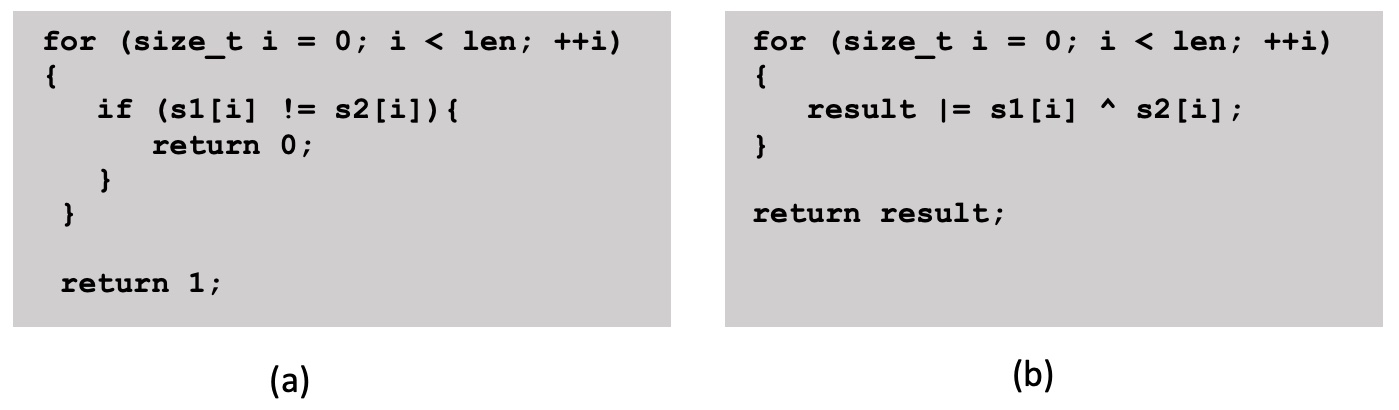
\includegraphics[width=.9\textwidth]{chapters/chapter3/image/string.jpg}
  \caption[Short caption for Table of Figures]{String Comparison}
  \label{fig:string}
\end{figure}

    \item \textbf{diamond:} This program features two branching instructions dependent on secret values and one independent branch.

    \item \textbf{loop:} The program contains a loop that relies on a condition with public data and includes a secret-dependent branch within the loop body. 
    
    \item \textbf{secure\_loop:} In contrast, this code employs bitwise operations to eliminate the need for a conditional branch.
    
    \item \textbf{multifork:} In this program, a switch statement evaluates the value of a secret variable and compares it against multiple cases. 
    
    \item \textbf{ifthenloop \& ifthenloop\_nop\_padded:} These programs involve a branch dependent on secret data and a loop with a public variable in its condition, executed if the branch is taken. In the 'ifthenloop\_nop\_padded' version, additional dummy instructions are introduced to ensure a balanced execution across both branches.  
    
    \item \textbf{ifthenlooplooptail:} This program introduces nested secret-dependent branches and loops, creating a more intricate control flow to thoroughly test \gls{SCF}\textsuperscript{ARM}.

\end{itemize}


\begin{sidewaystable}
    \centering
		\caption{ Evaluation results for \gls{SCF}\textsuperscript{ARM} on the benchmark suite. For each compiled example program, we give an indication for C program complexity (LOC = lines of code, CFG Size = number of nodes in the program’s Control Flow Graph), execution time of \gls{SCF}\textsuperscript{ARM}, and list the vulnerabilities found by \gls{SCF}\textsuperscript{ARM}.}
  
		\label{tab:eval3}
  
		\begin{tabular}{llcccccc}
			\hline
			\textbf{Benchmark} &\textbf{LOC}
& \textbf{CFG}& \textbf{\gls{SCF}\textsuperscript{ARM}}& \textbf{Timing}& \textbf{Nemesis} &\textbf{BUSted} & \textbf{Storage}\\ 
		    {} &{} & \textbf{Size}& \textbf{exec time}& \textbf{Channel}& \textbf{Vulnerability} & \textbf{Vulnerability} & \textbf{Channel}\\ 
			\hline

busted & 14 & 20 & 3.042s & $\times$ & \checkmark & \checkmark & \checkmark \\ 

busted-free & 15 & 21 & 3.725s & \checkmark & \checkmark & $\times$ & \checkmark \\   

strcmp & 10 & 34 & 4.563s & \checkmark & \checkmark & \checkmark &      $\times$ \\ 

constant\_time\_strcmp & 13 & 39 & 2.564s & $\times$ & $\times$ &       $\times$ & $\times$ \\ 

diamond & 20 & 35 & 4.762s & \checkmark & \checkmark & \checkmark & \checkmark \\ 

loop & 16 & 49 & 3.330s & \checkmark &  \checkmark & \checkmark & \checkmark \\ 

secure\_loop & 22 & 58 & 4.902s & $\times$ & $\times$ & $\times$ & \checkmark \\ 

fork & 7 & 19 & 3.269s & \checkmark & \checkmark & \checkmark & \checkmark \\ 

fork\_nop\_padded & 12 & 24 & 3.769s & $\times$ & \checkmark & \checkmark & \checkmark \\ 

indirect & 20 & 29 & 3.460s & \checkmark & \checkmark & \checkmark & \checkmark \\ 

multifork & 15 & 34 & 4.013s & \checkmark & \checkmark & \checkmark & \checkmark \\

branchless\_multifork & 8 & 42 & 2.713s & $\times$ & $\times$ & $\times$ & \checkmark \\ 

ifcompound & 22 & 33 & 4.480s & \checkmark & \checkmark & \checkmark & \checkmark \\

call & 19 & 29 & 2.762s & $\times$ & $\times$  & $\times$ & \checkmark\\
		 		   
ifthenloop & 20 & 43 & 4.476s & \checkmark & \checkmark & \checkmark & $\times$ \\ 

ifthenloop\_nop\_padded & 25 & 50 & 4.608s & $\times$ & \checkmark & \checkmark & $\times$ \\

ifthenloopif & 28 & 74 & 6.890s & \checkmark & \checkmark & \checkmark & $\times$ \\ 

ifthenlooploop & 28 & 67 &  7.580s & \checkmark & \checkmark & \checkmark & $\times$ \\

ifthenlooplooptail & 38 & 110 & 8.136s & \checkmark & \checkmark & \checkmark & $\times$ \\

multiply & 5 & 12 & 3.789s & $\times$ & $\times$ & $\times$ & \checkmark \\
	   		   
		   \hline
		\end{tabular}
\end{sidewaystable}

In Table \ref{tab:eval3}, we present the experimental outcomes obtained by applying \gls{SCF}\textsuperscript{ARM} to the benchmark. Our results showcases that \gls{SCF}\textsuperscript{ARM} effectively analyzes intricate binaries designed for ARM Cortex-M23. The tool not only adeptly identifies a spectrum of side-channel vulnerabilities but also demonstrates its efficiency in swiftly and accurately detecting sensitive data leakage. Keep in mind that utilizing branch balancing or constant-time programming by itself cannot entirely eliminate the risk of unintended information leakage within a program. In such instances, it becomes imperative to take additional measures, such as securely storing program outputs in a designated protected memory space or returning them in an encrypted format. These precautions provide an extra layer of security, effectively mitigating the possibility of sensitive information being unintentionally exposed to attackers, even when employing the mentioned programming techniques.

\subsection{Discussion}

\textbf{Soundness.} In this study, we emphasize the paramount importance of soundness in our symbolic taint-tracking approach, aiming to establish credible security assurances for Cortex-M23 programs. Central to our methodology is the meticulous consideration of the execution time required for instructions on a Cortex-M23 microcontroller. It is noteworthy that in the absence of sophisticated architectural features such as paging, caches, or out-of-order instruction pipelining, the time taken for instruction execution is wholly deterministic.

The foundation of our proposed approach rests on the predictability of an instruction's execution time, a characteristic intrinsic to Cortex-M23 microcontrollers. This inherent determinism serves as a cornerstone for the soundness of our approach, enabling precise prediction of an instruction's execution time. Consequently, programs certified by our \gls{SCF}\textsuperscript{ARM} are inherently fortified against timing-side-channel vulnerabilities.

\textbf{Nemesis Detection.} As of our current knowledge, there have been no reported instances of a Nemesis attack being executed on an ARM Cortex-M microcontroller. Nevertheless, it is important to note that the ARM Cortex-M23 possesses all the necessary prerequisites for a successful Nemesis attack. In general, the Cortex-M23 processor tends to complete the current instruction before handling an interrupt. This behavior, known as a "late-arriving interrupt" model, means that if an interrupt is pending and becomes active during the execution of an instruction, the processor finishes that instruction before switching to the Interrupt Service Routine (\gls{ISR}). However, the precise handling may vary depending on the specific microcontroller implementation and the configuration of the Nested Vectored Interrupt Controller (NVIC) that manages interrupts in the Cortex-M series.

This interrupt handling mechanism introduces timing variations between interrupted instructions, which could be leveraged by an attacker to distinguish between secret-dependent branches. Furthermore, in our attacker model, the adversary has the capability to control a timer device and closely monitor \gls{ISR}s, roughly resembling a configuration conducive to launching a Busted attack \cite{busted}.

\textbf{Path explosion.} Similar to other symbolic-execution tools, \gls{SCF}\textsuperscript{ARM} encounters the widely recognized challenge of state explosion, particularly evident when dealing with larger binaries. The exponential increase in path complexities renders exhaustive exploration practically infeasible, potentially leaving vulnerabilities undetected within unexplored paths. Additionally, it is noteworthy that Angr, the foundational symbolic execution framework for \gls{SCF}\textsuperscript{ARM}, introduces an inherent unsoundness by potentially concretizing values during symbolic execution. These challenges are orthogonal to the core contribution of this paper. Addressing the issue of path explosion and enhancing the soundness of symbolic execution tools are recognized as critical engineering tasks. While beyond the scope of the current study, we acknowledge them as essential aspects deserving of attention in future work.



%\section{Related Work}\label{sec:related3}

\paragraph{Side-channel Attacks on TrustZone-M.}
 
 Extensive research has been conducted on microarchitectural timing channels \cite{timingattack}, notably introduced by Kocher \cite{Kocher96}, gaining widespread attention following the disclosure of Spectre \cite{spectre} and Meltdown \cite{meltdown}. However, exploration into side-channel attacks within TEE context is a relatively recent endeavor. Several authors \cite{loadstep, truspy, Bypassed, Qualcomm, vanbulckphdthesis, gross2019breaking, surveyonTEE} have raised concerns regarding software side-channel vulnerabilities in higher-end TEEs like Arm TrustZone. Additionally, research efforts on Microcontroller Units (MCUs) \cite{Nemesis, marton, busted, returntononsecure, oflynn2019ondevice, barenghi2021cortexm, gnad2019leakynoise} have investigated the potential for information leakage through software-based side-channels. For instance, Gnad et al. in \cite{gnad2019leakynoise} capitalized on the correlation between ADC noise and MCU power consumption in Cortex-M4, utilizing software power consumption traces to extract secret keys from an AES implementation. Similarly, O'Flynn and Alex Dewar in \cite{oflynn2019ondevice} exploited the ADC in a SAM L11 (Cortex-M23) MCU, executing a remote power side-channel attack to bypass TrustZone-M protection and retrieve a secret key. In contrast to power side-channel attacks, Nemesis attack by Van Bulck et al. \cite{Nemesis} exploits the CPU's interrupt mechanism to extract instruction timings from MSP430 MCUs. In \cite{marton}, the authors leverage minor timing variations in unprivileged DMA requests, arising from contention on the shared memory bus within openMSP430 MCUs, to acquire a memory access trace of a victim program. Likewise, BUSted \cite{busted} represents a type of side-channel attack utilizing timing discrepancies on the MCU bus interconnect to bypass the security assurances provided by memory protection primitives in Armv8-M MCUs with TrustZone-M.
 
\paragraph{Microarchitectural Timing Side Channels Static Analysis.} There exists substantial literature on timing side channel detection employing ML models \cite{MLforSC, chiappetta2016realtime, allaf2017comparison}, dynamic taint analysis \cite{graa2017detection}, fuzzing \cite{nilizadeh2018diffuzz}, Abstract interpretation \cite{kopf2012automatic, doychev2015cacheaudit}, Logical reduction \cite{chen2017precise}, type-based solutions \cite{MantelAVR, scfmsp, barthe2014system, rodrigues2016sparse, zhang2012languagebased, lux2011tool}, and several other methodologies \cite{timingattack, akram2020sherlock, szefer2019survey}. Our focus will be on approaches that bear direct relevance to our research. Köpf et al. \cite{kopf2012automatic} proposed an approach to automatically derive upper bounds on cache leakage within cryptographic executables. Subsequently, CacheAudit \cite{doychev2015cacheaudit} expanded upon their research by enhancing abstractions and precision. It uses static analysis for cache side channels to derive formal, quantitative security guarantees for a comprehensive set of side-channel adversaries, based on observing cache states, traces of hits and misses, and execution times. Chen et al. \cite{chen2017precise} introduced Themis, an innovative end-to-end static analysis tool tailored for Java applications. Themis utilizes Quantitative Cartesian Hoare Logic (QCHL) to verify $\epsilon$-bounded noninterference, enabling the detection of intricate resource-usage side-channel vulnerabilities within real-world Java programs. 

FlowTracker \cite{rodrigues2016sparse} offers the capability to statically trace data dependencies, identifying possible timing leaks in LLVM programs. By leveraging the presumption of LLVM code being in Static Single Assignment (SSA) format, the tool computes control dependencies through a sparse analysis method, negating the need to construct the entire Program Dependency Graph. Barthe et al. \cite{barthe2014system} proposed an assembly-level type system to verify the constant-time policy. Zhang et al. \cite{zhang2012languagebased} introduced a language-based approach for a basic While-language, aiming to track side-channel leaks. The authors suggested a cooperative model between hardware and software to mitigate covert timing channel. Side Channel Finder (\ac{SCF}) \cite{lux2011tool} checks secret-dependent loops and branching using a type system for static detection of timing channels in Java. In our prior work \cite{scfmsp}, we proposed a security type system designed for statically analyzing MSP430 binaries. This system ensures the absence of timing leaks, Nemesis-style vulnerabilities, and unintended information flow through covert storage channel. To enhance the accuracy of our analysis from previous research and expand our capability to trace information flow across TrustZone-provided protection domains, this study employs a symbolic execution-based analysis. This allows for meticulous control over memory operations, refining the precision of our analysis.

\paragraph{Symbolic Execution.} Some works \cite{binsec, pitchfork, sung2018canal, chattopadhyay2018symbolic, brotzman2019casym, brennan2018symbolic, yavuz2022encider, pasareanu2016multi, bang2016string} have, furthermore, focused on detecting microarchitectural side-channel vulnerabilities using symbolic execution. For instance, Bang et al. \cite{bang2016string} use symbolic execution, string analysis, and model counting to quantify leakage for a particular type of side channel. Pasareanu et al. \cite{pasareanu2016multi} proposed a symbolic execution approach for side-channels detection and quantification. They measure side-channel leakage by creating specific public inputs that trigger maximum leakage. This is accomplished through Max-SMT solving applied to the constraints derived from symbolic execution. ENCIDER \cite{yavuz2022encider} employs dynamic symbolic execution and taint analysis to uncover timing and cache side-channel vulnerabilities within Intel SGX applications. It decomposes side-channel requirements based on the bounded non-interference property and implements byte-level information flow tracking through API modeling. CoCo-Channel \cite{brennan2018symbolic} employs taint analysis to detect secret-dependent conditional statements within Java programs. It assigns symbolic cost expressions to various program paths and utilizes symbolic execution to identify and report paths demonstrating secret-dependent timing behavior.

Additionally, various other studies \cite{sung2018canal, chattopadhyay2018symbolic, brotzman2019casym} leverage symbolic execution to derive a symbolic cache model and verify that the cache behavior remains independent of sensitive data. Scalability concerns often hinder symbolic execution. Daniel et al. \cite{binsec} introduced an automatic, efficient binary-level verification method tailored for constant-time analysis. This method conducts both bug identification and bounded verification on practical cryptographic implementations. Employing relational symbolic execution with specialized optimizations in information flow and binary-level analysis, their approach maximizes shared information between executions following the same path. Pitchfork \cite{pitchfork} unites symbolic execution and dynamic taint tracking to accurately propagate secret taints across all execution paths, highlighting tainted branch conditions or memory addresses. Notably, Pitchfork can analyze protocol-level code by abstracting the implementation details of primitives through function hooks, allowing separate analysis of these components. 

Developing constant-time code presents complexity due to the need for intricate low-level operations that diverge from conventional programming practices. Maintaining this approach proves challenging as compiler optimizations often fail to preserve such implementations. Moreover , the vulnerability revealed in the attack on the constant-time implementation applied to the Curve25519 elliptic curve \cite{kaufmann2016constanttime} highlights the error-prone nature of writing such code. This work explores a purely static method for identifying timing side channels by integrating symbolic execution and taint analysis. Our prototype, \ac{SCF}\textsuperscript{ARM}, was developed to verify ARMv8-M binaries for potential side channel vulnerabilities. To the best of our knowledge, this represents the first static analysis tool capable of automatically detecting timing side channels, Nemesis, BUSted, and covert storage leakage, within ARM-M binaries.

%\section{Conclusions and Future Directions}

We presented \tool{} as a new tool for the automated detection of
microarchitectural side channels, specifically targeting timing side
channels, Nemesis, BUSted attacks, and information leakage, in TrustZone-M
applications. Our work relies on the predictability of execution times on
Cortex-M processors, which allowed us to develop a symbolic taint-tracking
approach for timing-sensitive information flow analysis with a high degree
of precision. We applied \tool{} to a range of synthetic and real-world
benchmarks. The outcomes of these experiments illustrate the tool's
capability to identify a spectrum of side-channel vulnerabilities, enabling
developers to assess and mitigate these vulnerabilities. To the best of our
knowledge \tool{} is the first sied-channel detetion tool for compiled
ARMv8-M programs and we make our tool and benchmarks publicly available.

Several avenues for future research emerge from this work. Firstly, we aim
to enhance the comprehensiveness of our framework by extending its coverage
to encompass the entire ARMv8-M instruction set. We intend to conduct a
comprehensive evaluation of \tool{} by applying it to off-the-shelf
TrustZone-M programs and scrutinizing its performance in real-world
implementations of cryptographic libraries, such as wolfSSL~\cite{wolfssl}.
Moreover, in pursuit of efficiency improvements, the incorporation of
state-merging~\cite{kuznetsov2012efficient} or path prioritization
strategies~\cite{baldoni2018survey, li2013steering} would be useful.




\bibliographystyle{plain}
\bibliography{paper.bib}

\appendices

\end{document}
